\documentclass[a4,compress]{beamer}

\usepackage{beamerthemesplit}

\usepackage{amsmath, amsfonts, amssymb}
\usepackage{amsthm}
\usepackage{mathtools}
\usepackage{physics}

\usepackage{graphicx}
\graphicspath{{figures/}}

\usepackage[utf8]{inputenc}

\usepackage{times}
\usepackage[T1]{fontenc}

\usepackage[english]{isodate}

% Theorems and definitions

\theoremstyle{plain}
\newtheorem*{theorem*}{Theorem}

\theoremstyle{definition}
\newtheorem*{def*}{Definition}

% Begin presentation

\mode<presentation>
{
  \usetheme{Warsaw}
  \setbeamercovered{transparent}
}

\AtBeginSection[]
{
  \begin{frame}
    \frametitle{Outline}
    \tableofcontents[currentsection]
  \end{frame}
}

\addtobeamertemplate{navigation symbols}{}{%
    \usebeamerfont{footline}%
    \usebeamercolor[fg]{footline}%
    \hspace{1em}%
    \insertframenumber/\inserttotalframenumber
}

\addtobeamertemplate{title page}{
\includegraphics[width=1.3cm]{logo/unibuc} \hfill 
\includegraphics[width=1.6cm]{logo/fizica}}{}

\title[Title (appears on every slide)]{Full title at the beginning}
\subtitle{Master Thesis}

\author{
  Prenume NUME \\
   \hspace{6cm} {\small	Scientific Advisers:} \\
   \hspace{6.35cm} {\small Prof.~dr.~Virgil BĂRAN}
}

\institute[Universitatea din București]
{
  Universitatea din București \\
  Facultatea de Fizică
}
\date{\small Bucharest, 29 \printdayoff\today}

\begin{document}

%%%%%%%%%%%%%%%%%%%%%%%%%%%% slide 1 %%%%%%%%%%%%%%%%%%%%%%%%%%%%

\begin{frame}[plain]
 \titlepage
\end{frame}

%%%%%%%%%%%%%%%%%%%%%%%%%%%% slide 2 %%%%%%%%%%%%%%%%%%%%%%%%%%%%

\begin{frame}{Outline}
  \tableofcontents[]
\end{frame}

\section[Intro]{Introduction}

%%%%%%%%%%%%%%%%%%%%%%%%%%%% slide 3 %%%%%%%%%%%%%%%%%%%%%%%%%%%%

\begin{frame}
  \begin{itemize}
    \item The aim of this thesis is to study something.
  \end{itemize}
\end{frame}

\section[Short title]{Section title}

\subsection{Subsection title}

%%%%%%%%%%%%%%%%%%%%%%%%%%%% slide 4 %%%%%%%%%%%%%%%%%%%%%%%%%%%%

\begin{frame}
  \begin{itemize}
    \item Item and formula
    \begin{equation*}
      \label{eq:hamilton-jacobi-first}
      \mathcal{H}(q_1,\dotsc,q_n,\pdv{S}{q_1},\dotsc,\pdv{S}{q_n},t) + \pdv{S}{t} = 0
    \end{equation*}
    \item Formulae aligned on one line
    \begin{align*}
      I_k = \frac{1}{2\pi}\oint p_k \dd{q_k}, &&
      \theta_k = \omega_k(I_k) \Delta t
    \end{align*}
    \item An item with some text. And an \emph{emphasized} word.
    \item Don't write too much on a slide.
  \end{itemize}
\end{frame}

%%%%%%%%%%%%%%%%%%%%%%%%%%%% slide 5 %%%%%%%%%%%%%%%%%%%%%%%%%%%%

\begin{frame}{Frame title}
  \begin{itemize}
    \item Canonical perturbation theory exploits
    the special properties of action-angle variables.
    \[
      \mathcal{H}(I, \theta) = \mathcal{H}_0(I) + \epsilon \mathcal{H}_1(I, \theta).
    \]
    \item The basic idea of canonical perturbation theory is to find the new set of
    action-angle variables (\(J, \varphi\)) for the perturbed system
    \(\mathcal{H}(I,\theta)\) such that there is a canonical transformation to
    a new Hamiltonian which depends only on $J$, that is
    \[
    \mathcal{H}(I,\theta) \to K(J).
    \]
  \end{itemize}

\end{frame}

%%%%%%%%%%%%%%%%%%%%%%%%%%%% slide 6 %%%%%%%%%%%%%%%%%%%%%%%%%%%%

\subsection[Short subs.]{Another subsection}

\begin{frame}{Numbered lists}
  \begin{enumerate}
    \item First item
    \item Do not hardcode numbers in titles or section names. The name should be descriptive. The same applies
			to labels.
    \item For quotes you should use ``this''.
	\item You can split the frame in columns. See for example the next frame which features two images side by side
  \end{enumerate}
\end{frame}

%%%%%%%%%%%%%%%%%%%%%%%%%%%% slide 7 %%%%%%%%%%%%%%%%%%%%%%%%%%%%

\begin{frame}
  \begin{columns}[c]
   \begin{column}{0.5\textwidth}
     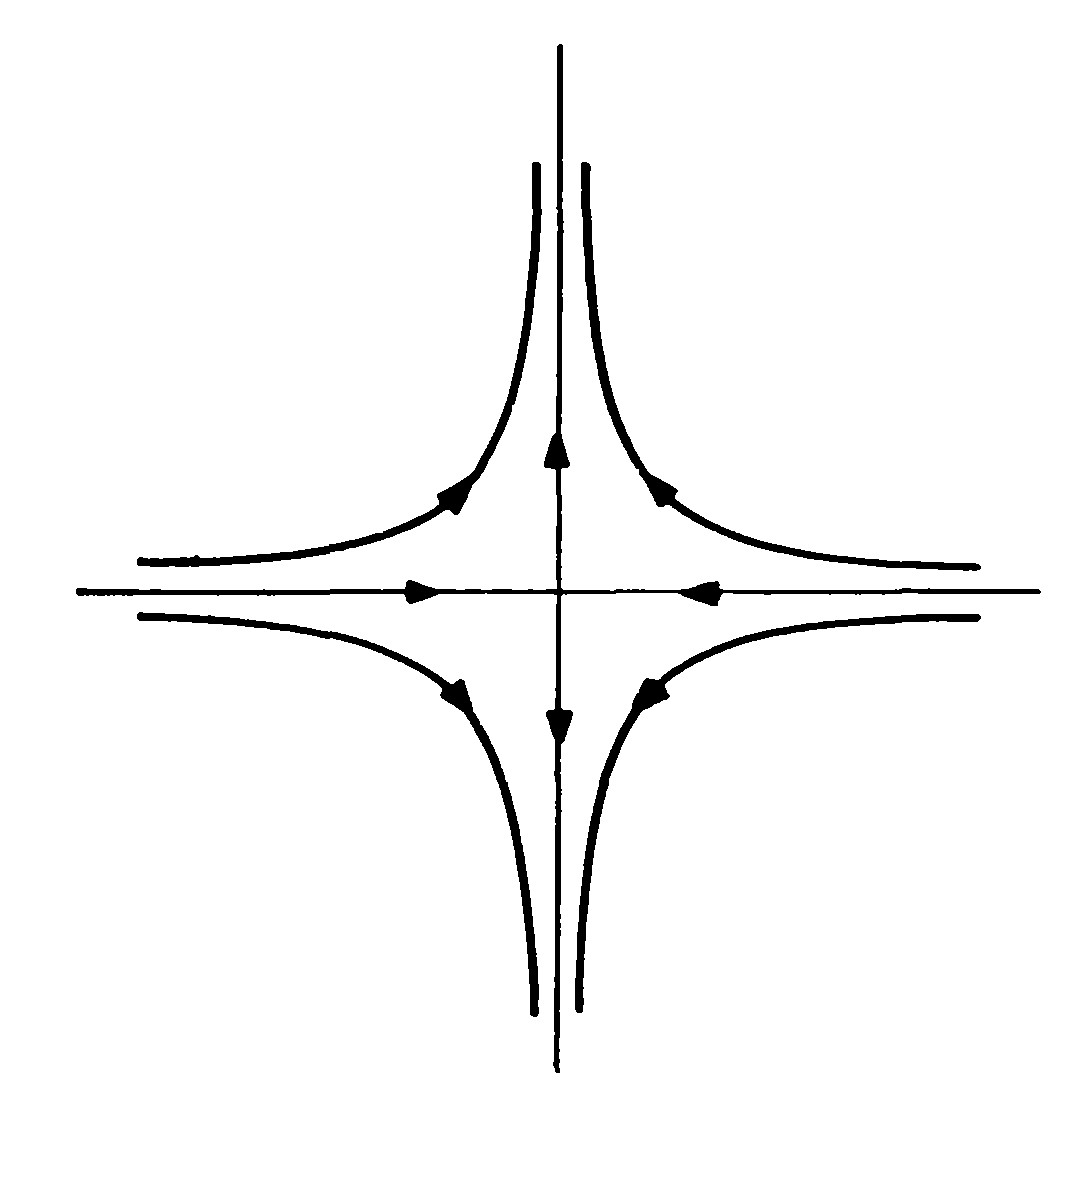
\includegraphics[width=\textwidth]{hyperbolic}  
   \end{column}
   \begin{column}{0.5\textwidth}
     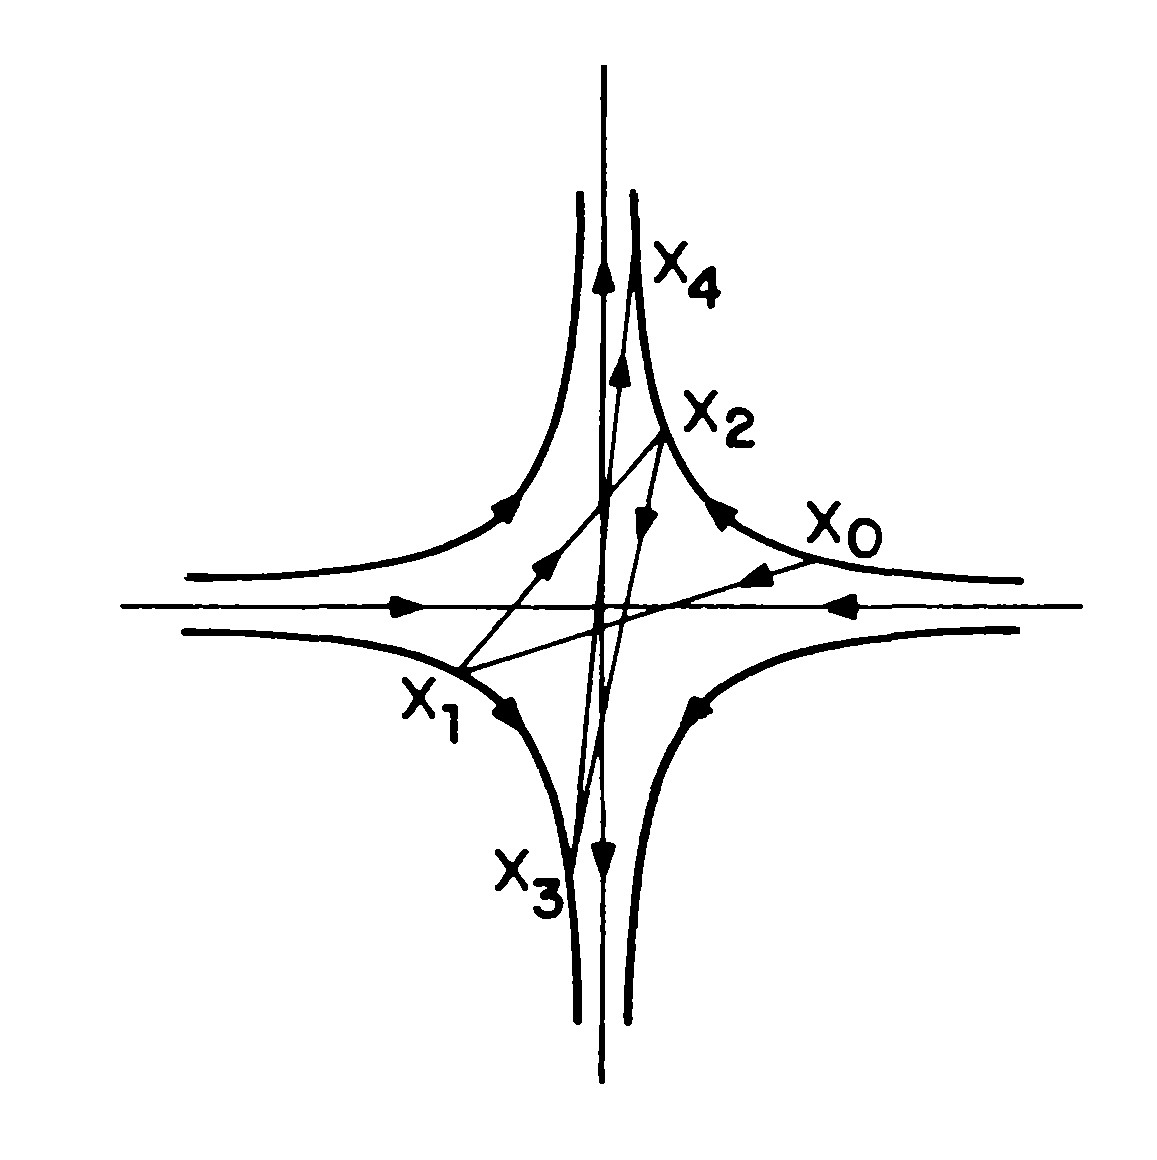
\includegraphics[width=\textwidth]{hyperbolic-reflection}
   \end{column}
 \end{columns}
\end{frame}

%%%%%%%%%%%%%%%%%%%%%%%%%%%% slide 8 %%%%%%%%%%%%%%%%%%%%%%%%%%%%

\begin{frame}
  \begin{itemize}
    \item This an example in which we intercalate an image with text without alignment
    \begin{equation*}
    \label{eq:parabolic-fixed-point}
    \begin{bmatrix}
      \var x_{i+1} \\
      \var y_{i+1}
    \end{bmatrix}
    =
    \begin{bmatrix}
      1 & c \\
      0 & 1
    \end{bmatrix}
    \begin{bmatrix}
      \var x_{i} \\
      \var y_{i}
    \end{bmatrix},
    \end{equation*}
    \begin{columns}[c]
     \begin{column}{0.5\textwidth}
       Here is some text to fill space: This corresponds to a
       translation parallel to the $x$-axis. This is known as a \emph{parabolic} fixed
       point.
     \end{column}
     \begin{column}{0.5\textwidth}
       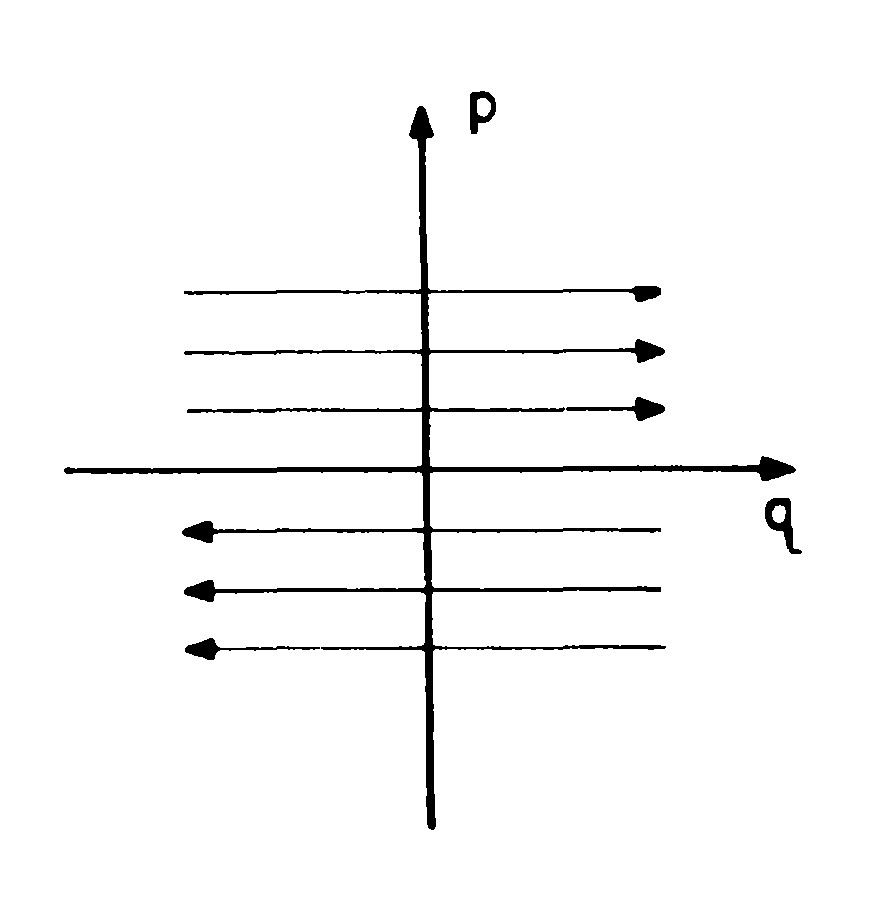
\includegraphics[width=\textwidth]{parabolic}
     \end{column}
   \end{columns}
  \end{itemize}
\end{frame}


%%%%%%%%%%%%%%%%%%%%%%%%%%%% slide 9 %%%%%%%%%%%%%%%%%%%%%%%%%%%%

\subsection[Last section]{The last section}

\begin{frame}
  \begin{itemize}
    \item If you can not fit all the short subsection titles maybe you have too many of them.
    \item We present an example of text aligned with an image. The solution is not perfect, but
	it works as a first order approximation. The width of the colums may need to be changed ny trial and error.
    \begin{columns}[T, onlytextwidth]
      \begin{column}{0.07\textwidth}

      \end{column}
      \begin{column}{0.65\textwidth}
        \item Text and formulae to fill space
        \[
        \begin{bmatrix}
          \varphi' \\
          I'
        \end{bmatrix}
        = T
        \begin{bmatrix}
          \varphi \\
          I
        \end{bmatrix},
        \]
        then \emph{every} point on \(\mathcal{C}\) is a fixed point of \(T^s\).
      \end{column}
      \begin{column}{0.3\textwidth}
        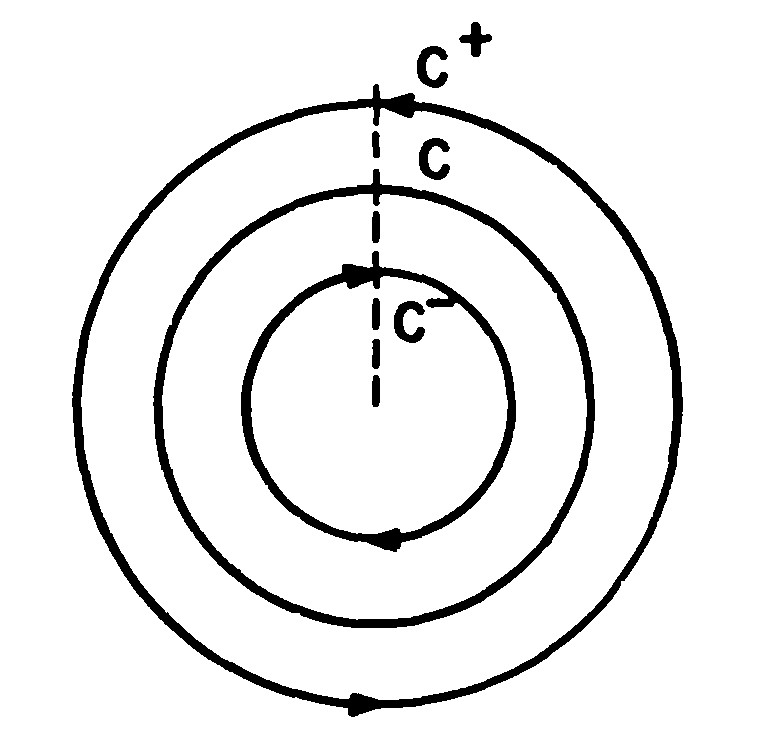
\includegraphics[width=\textwidth]{invariant-curves}
      \end{column}
    \end{columns}
  \end{itemize}
\end{frame}

%%%%%%%%%%%%%%%%%%%%%%%%%%%% slide 10 %%%%%%%%%%%%%%%%%%%%%%%%%%%%

\begin{frame}
  \begin{itemize}
    \item Now we consider an example with two items. As with the previous example the alignment is not perfect.
    \item And the space will be filled with random text: 
    the relative twists of \(\mathcal{C}^+\) and \(\mathcal{C}^-\) are preserved
    under \(T^s\).

    \begin{columns}[T, onlytextwidth]
      \begin{column}{0.05\textwidth}

      \end{column}
      \begin{column}{0.6\textwidth}
        \item If this is so, then there must be only one point between
        \(\mathcal{C}^+\) and \(\mathcal{C}^-\) whose angular coordinate \(\varphi\)
        is conserved under \(T^s\).
        \item In fact, along each radius (emanating from the centre)
        there must be one such point, so we can draw a curve $R$ of these points.
      \end{column}
      \begin{column}{0.3\textwidth}
        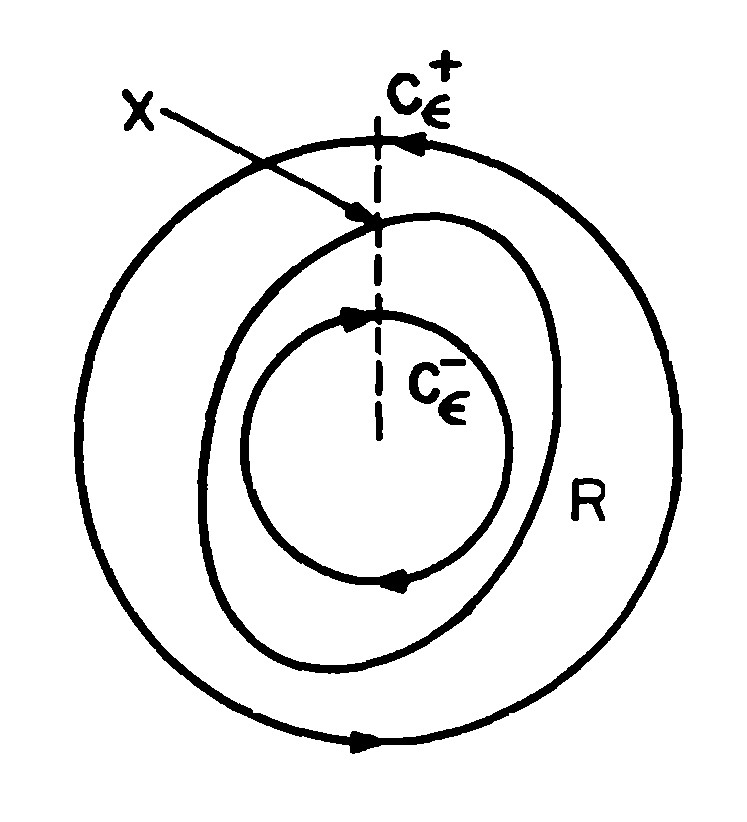
\includegraphics[width=\textwidth]{invariant-curves-perturbed}
      \end{column}
    \end{columns}
  \end{itemize}
\end{frame}

%%%%%%%%%%%%%%%%%%%%%%%%%%%% slide 11 %%%%%%%%%%%%%%%%%%%%%%%%%%%%

\begin{frame}
  \begin{itemize}
    \item An example with a centered figure
	\item below the items
  \end{itemize}
  \begin{center}
    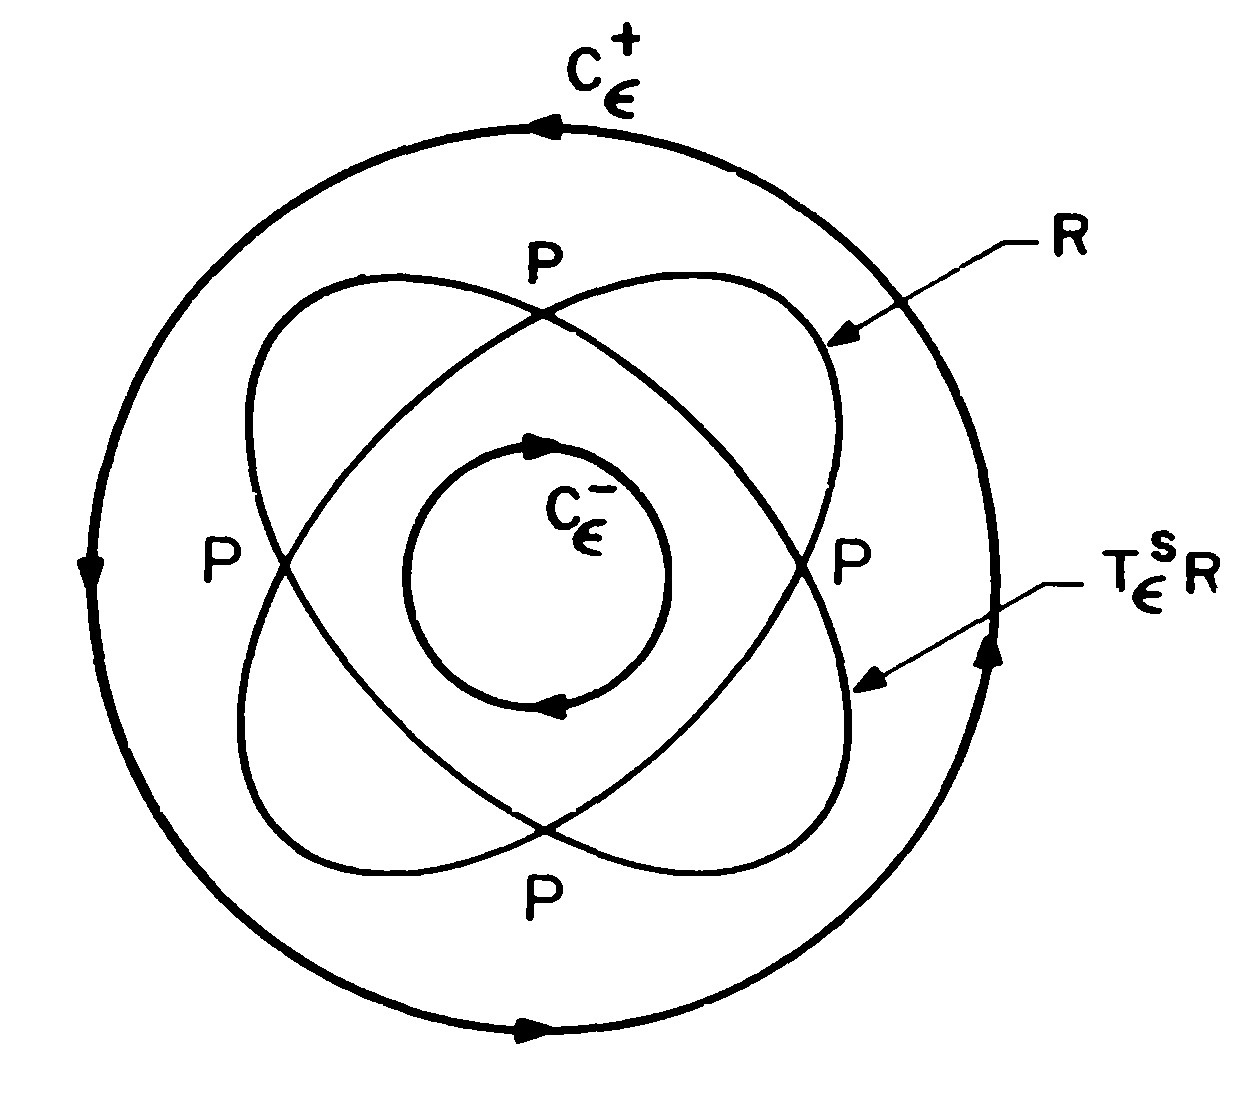
\includegraphics{fixed-points}
  \end{center}
\end{frame}

%%%%%%%%%%%%%%%%%%%%%%%%%%%% slide 12 %%%%%%%%%%%%%%%%%%%%%%%%%%%%

\begin{frame}
  \begin{itemize}
    \begin{columns}[T, onlytextwidth]
      \begin{column}{0.07\textwidth}

      \end{column}
      \begin{column}{0.6\textwidth}
        \item Now, finally we consider an example with a large image on the right side.
	    \item Notice that the items, while perfectly aligned on this frame, are not perfectly aligned
	    with the ones on the previous frame, but the alignment is very close to perfection.
        \item The dimensions of the columns in these examples should work in
        most cases. The third column is needed to align the items with the ones on the previous slide.
      \end{column}
      \begin{column}{0.4\textwidth}
        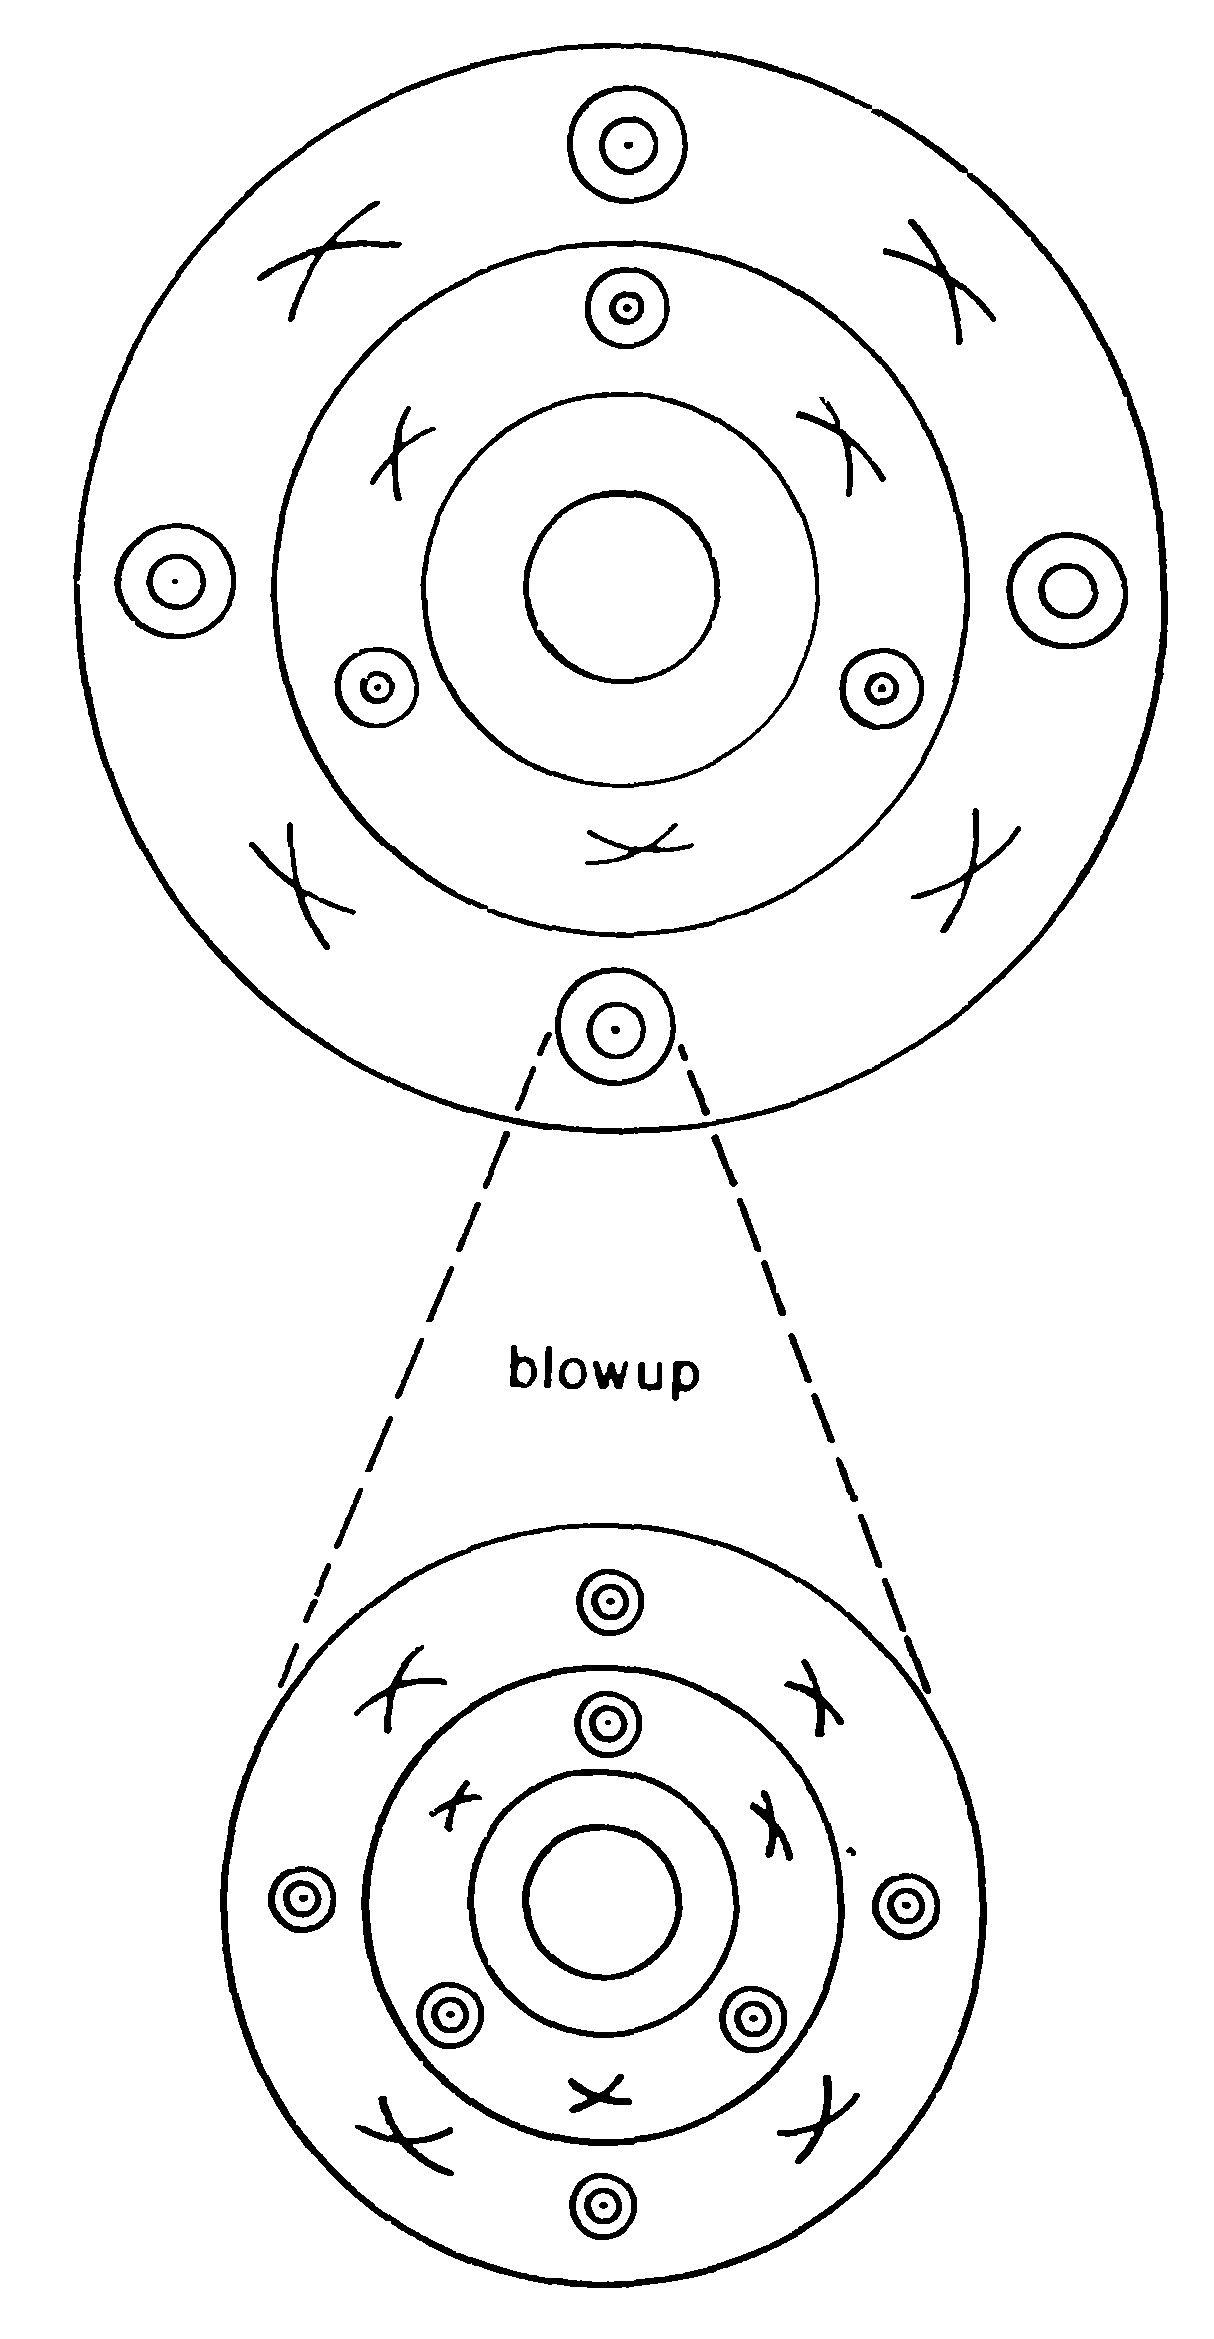
\includegraphics[width=.95\textwidth]{self-similar}
      \end{column}
    \end{columns}
  \end{itemize}
\end{frame}

%%%%%%%%%%%%%%%%%%%%%%%%%%%% slide 13 %%%%%%%%%%%%%%%%%%%%%%%%%%%%

\begin{frame}
  \begin{figure}[h]
    \centering
    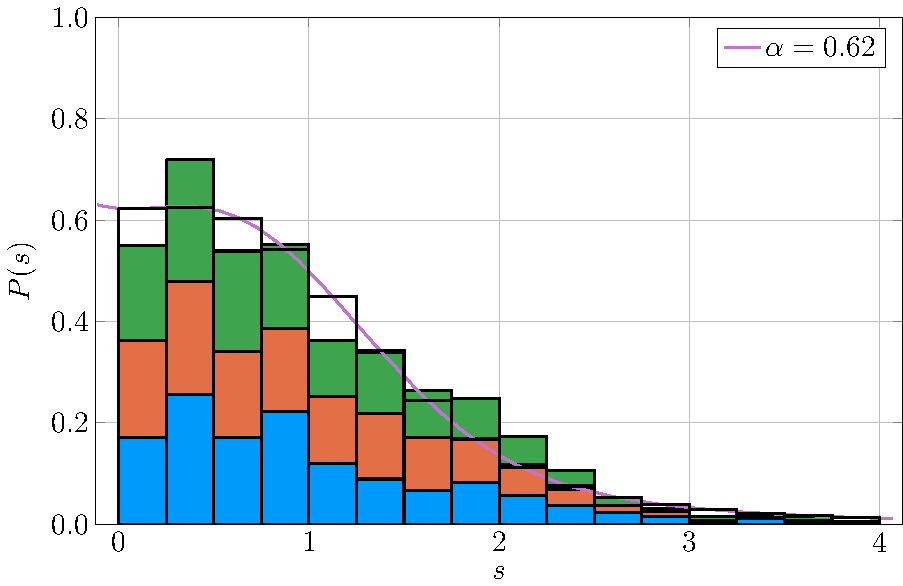
\includegraphics[width=\textwidth]{quantum/P(s)_slice_1}
    \caption{Full frame figure with caption}
  \end{figure}
\end{frame}

%%%%%%%%%%%%%%%%%%%%%%%%%%%% slide 14 %%%%%%%%%%%%%%%%%%%%%%%%%%%%

\section[Another section]{Another section}

\subsection{Some definitions}

\begin{frame}
  \begin{def*}[Joint probability]
    	Given two events $A$ and $B$, their joint probability, \(P(A \cap B)\), is
    	the probability of the two events to occur simultaneously.
  \end{def*}
  \begin{theorem*}[Pythagorean theorem]
    	This is a theorem about right triangles and can be summarised in the next equation 
	\[
	x^2 + y^2 = z^2
	\]
  \end{theorem*}
  \begin{itemize}
    \item Some examples of definitions.
  \end{itemize}
\end{frame}

%%%%%%%%%%%%%%%%%%%%%%%%%%%% slide 15 %%%%%%%%%%%%%%%%%%%%%%%%%%%%

\subsection[Subsection]{Subsection}

\begin{frame}{Block examples}
  \begin{block}{The block title}
    This content of the block appears like this.
  \end{block}
  \begin{block}{Another block with some text}
    This conjecture states that the nearest neighbour distribution of a quantum system
    with a classically chaotic counterpart is given by the Wigner distribution.
  \end{block}
\end{frame}

%%%%%%%%%%%%%%%%%%%%%%%%%%%% slide 16 %%%%%%%%%%%%%%%%%%%%%%%%%%%%

\subsection[Last]{Last subsection}

\begin{frame}
  \begin{itemize}
    \item This is an example of how to split a long formula
    \[
    \begin{split}
      \mathcal{H}(q_0,p_0,q_2,p_2) &= \frac{A}{2}(p_0^2 + p_2^2 + q_0^2 + q_2^2) \\
      &+ \frac{B}{\sqrt{2}}q_0(3q_2^2 - q_0^2)
      + \frac{D}{4}{(q_0^2 + q_2^2)}^2
    \end{split}
    \]
	\item Some empty frames will follow. Use them when creating new frames.
  \end{itemize}
\end{frame}

%%%%%%%%%%%%%%%%%%%%%%%%%%%% slide 17 %%%%%%%%%%%%%%%%%%%%%%%%%%%%

\begin{frame}{Empty frame with title}
  \begin{itemize}
    \item 
  \end{itemize}
\end{frame}

%%%%%%%%%%%%%%%%%%%%%%%%%%%% slide 18 %%%%%%%%%%%%%%%%%%%%%%%%%%%%

\begin{frame}
  \begin{itemize}
    \item 
  \end{itemize}
\end{frame}

%%%%%%%%%%%%%%%%%%%%%%%%%%%% slide 19 %%%%%%%%%%%%%%%%%%%%%%%%%%%%

\begin{frame}
  \begin{itemize}
    \item 
  \end{itemize}
\end{frame}

%%%%%%%%%%%%%%%%%%%%%%%%%%%% slide 20 %%%%%%%%%%%%%%%%%%%%%%%%%%%%

\begin{frame}
  \begin{itemize}
    \item 
  \end{itemize}
\end{frame}

\section{Conclusions}

%%%%%%%%%%%%%%%%%%%%%%%%%%%% slide 21 %%%%%%%%%%%%%%%%%%%%%%%%%%%%

\begin{frame}{Conclusions}
  \begin{itemize}
    \item Many hours of sleep were lost for this thesis.
    \item Replace this text with your actual conclusions.
    \item I hope this was useful.
  \end{itemize}
\end{frame}

\end{document}
